% !TEX root =  master.tex
\chapter{Ablaufplan}
\begin{figure}[H]
	\centering 
	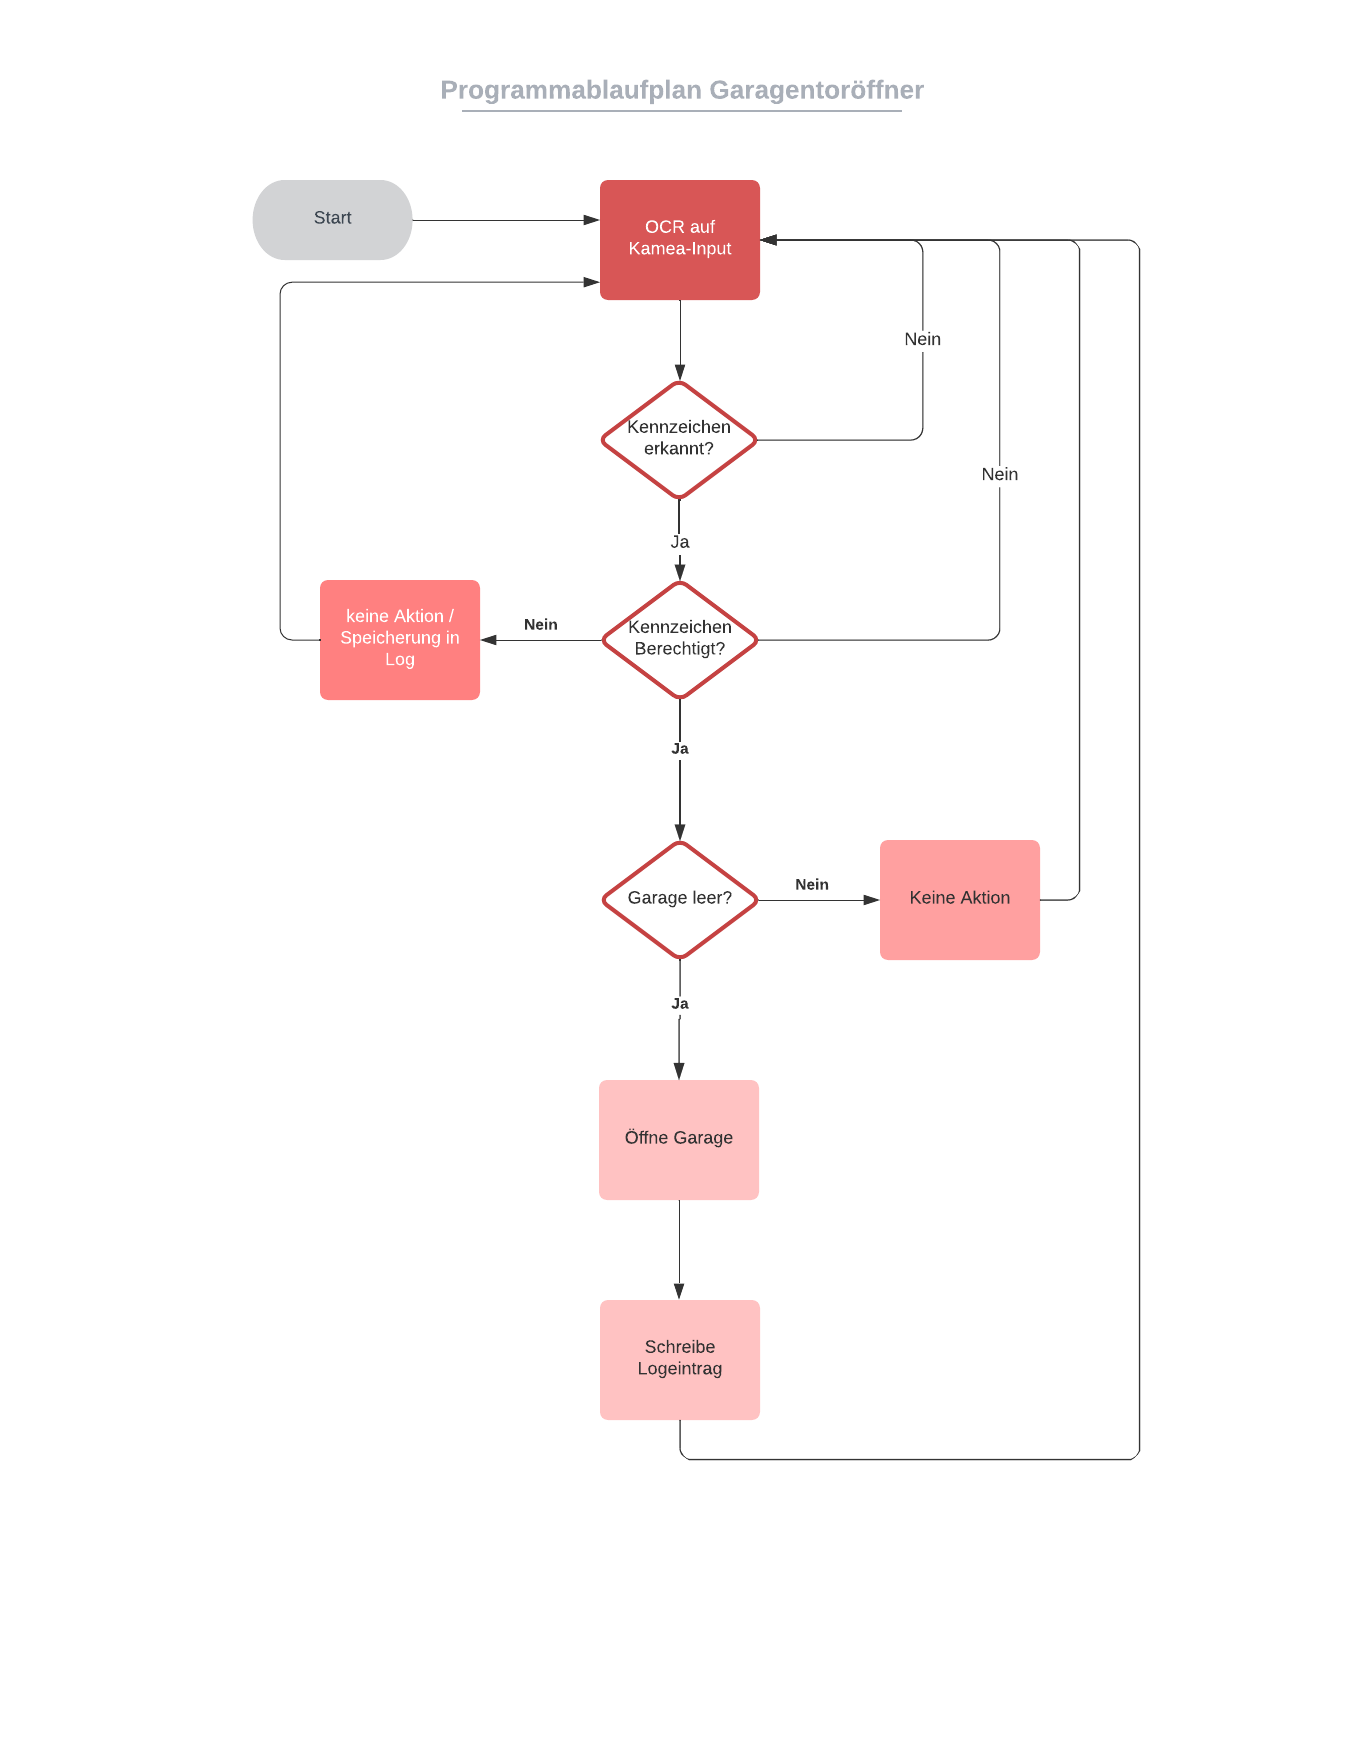
\includegraphics[scale=0.75]{\imagedir/Programmablaufplan.png}
	\captionsetup{format=hang}
	\caption[Programmablauf]{\label{Ablaufplan}Ablauf der Kennzeichenerkennungs-Schleife \\Quelle: Eigene Darstellung}
\end{figure}
\chapter{Schaltplan}
\begin{figure}[h]
	\centering
	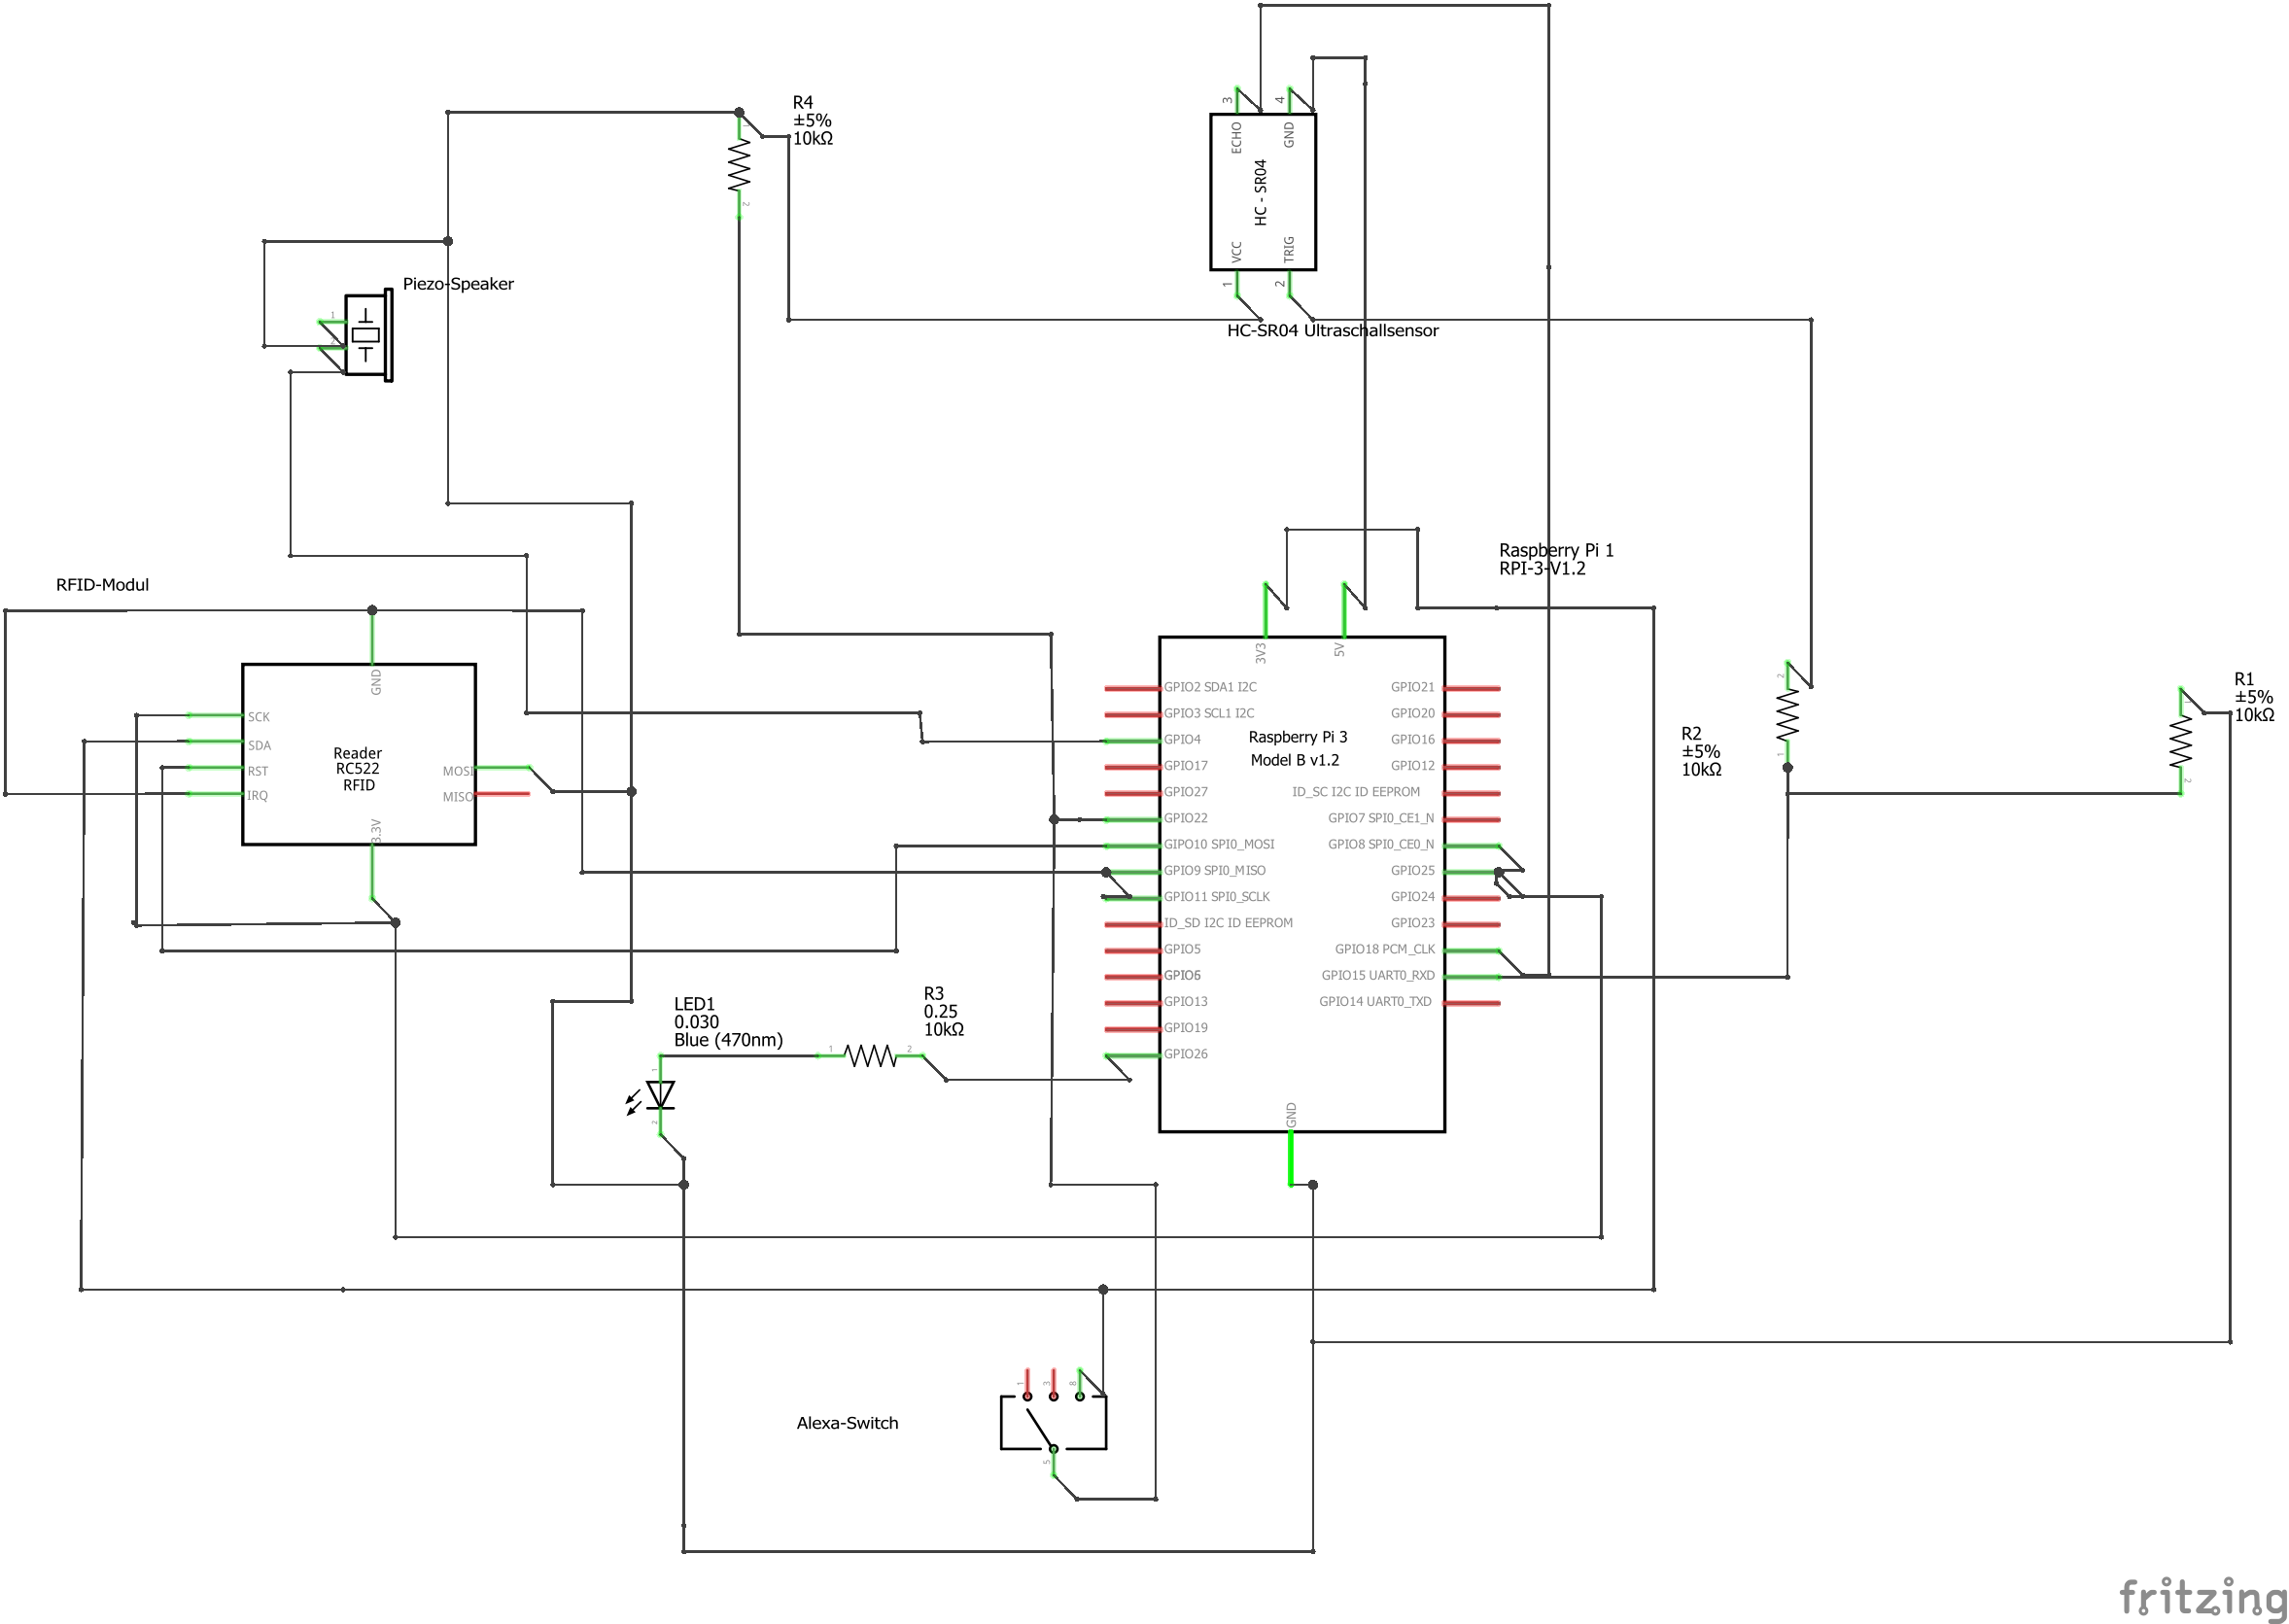
\includegraphics[width=1\linewidth]{img/SmartGarage_Schaltplan}
	\caption[Schaltplan]{Finaler Schaltplan aller Bauteile \\ Quelle: Eigene Darstellung}
	\label{Schaltplan}
\end{figure}

\chapter{Steckplan}
\begin{figure}[H]
	\centering 
	\label{Steckplan}
	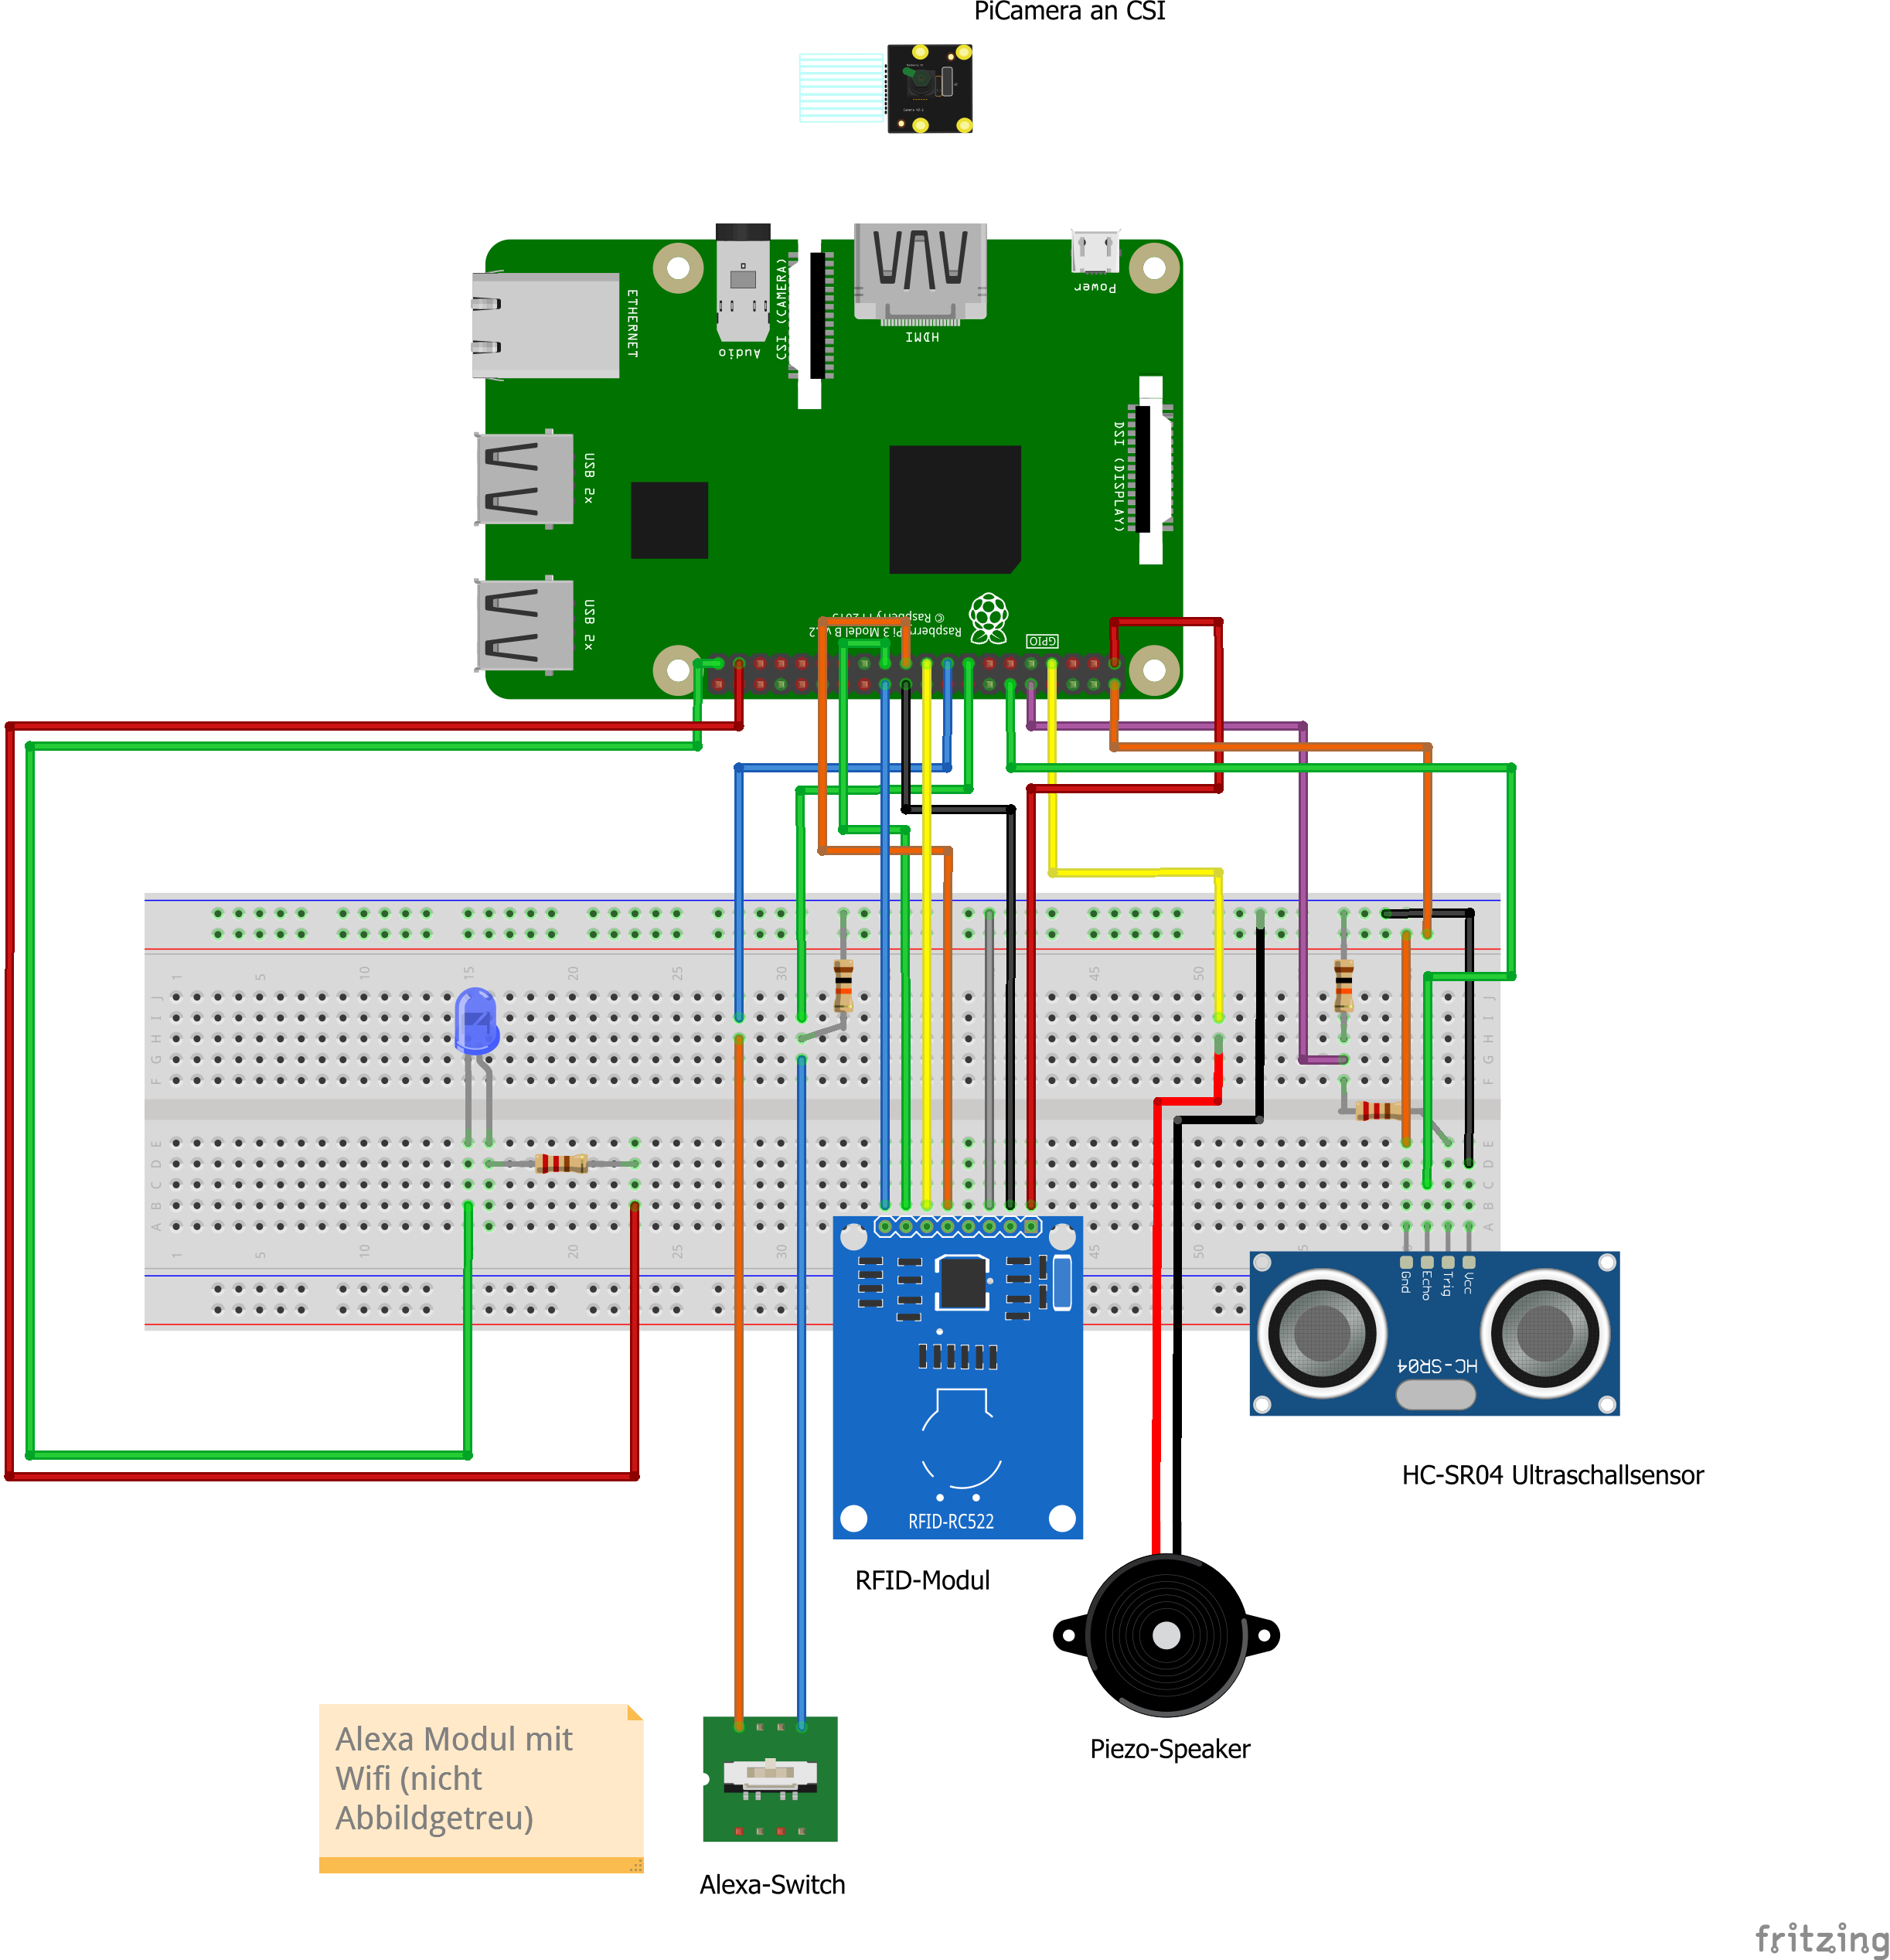
\includegraphics[scale=0.8]{\imagedir/SmartGarage.png}
	\captionsetup{format=hang}
	\caption[Steckplan groß]{Steckplan der gesamten Hardware \\Quelle: Eigene Darstellung}
\end{figure}
\chapter{Versuchsaufbau}
\begin{figure}
	\centering 
	
	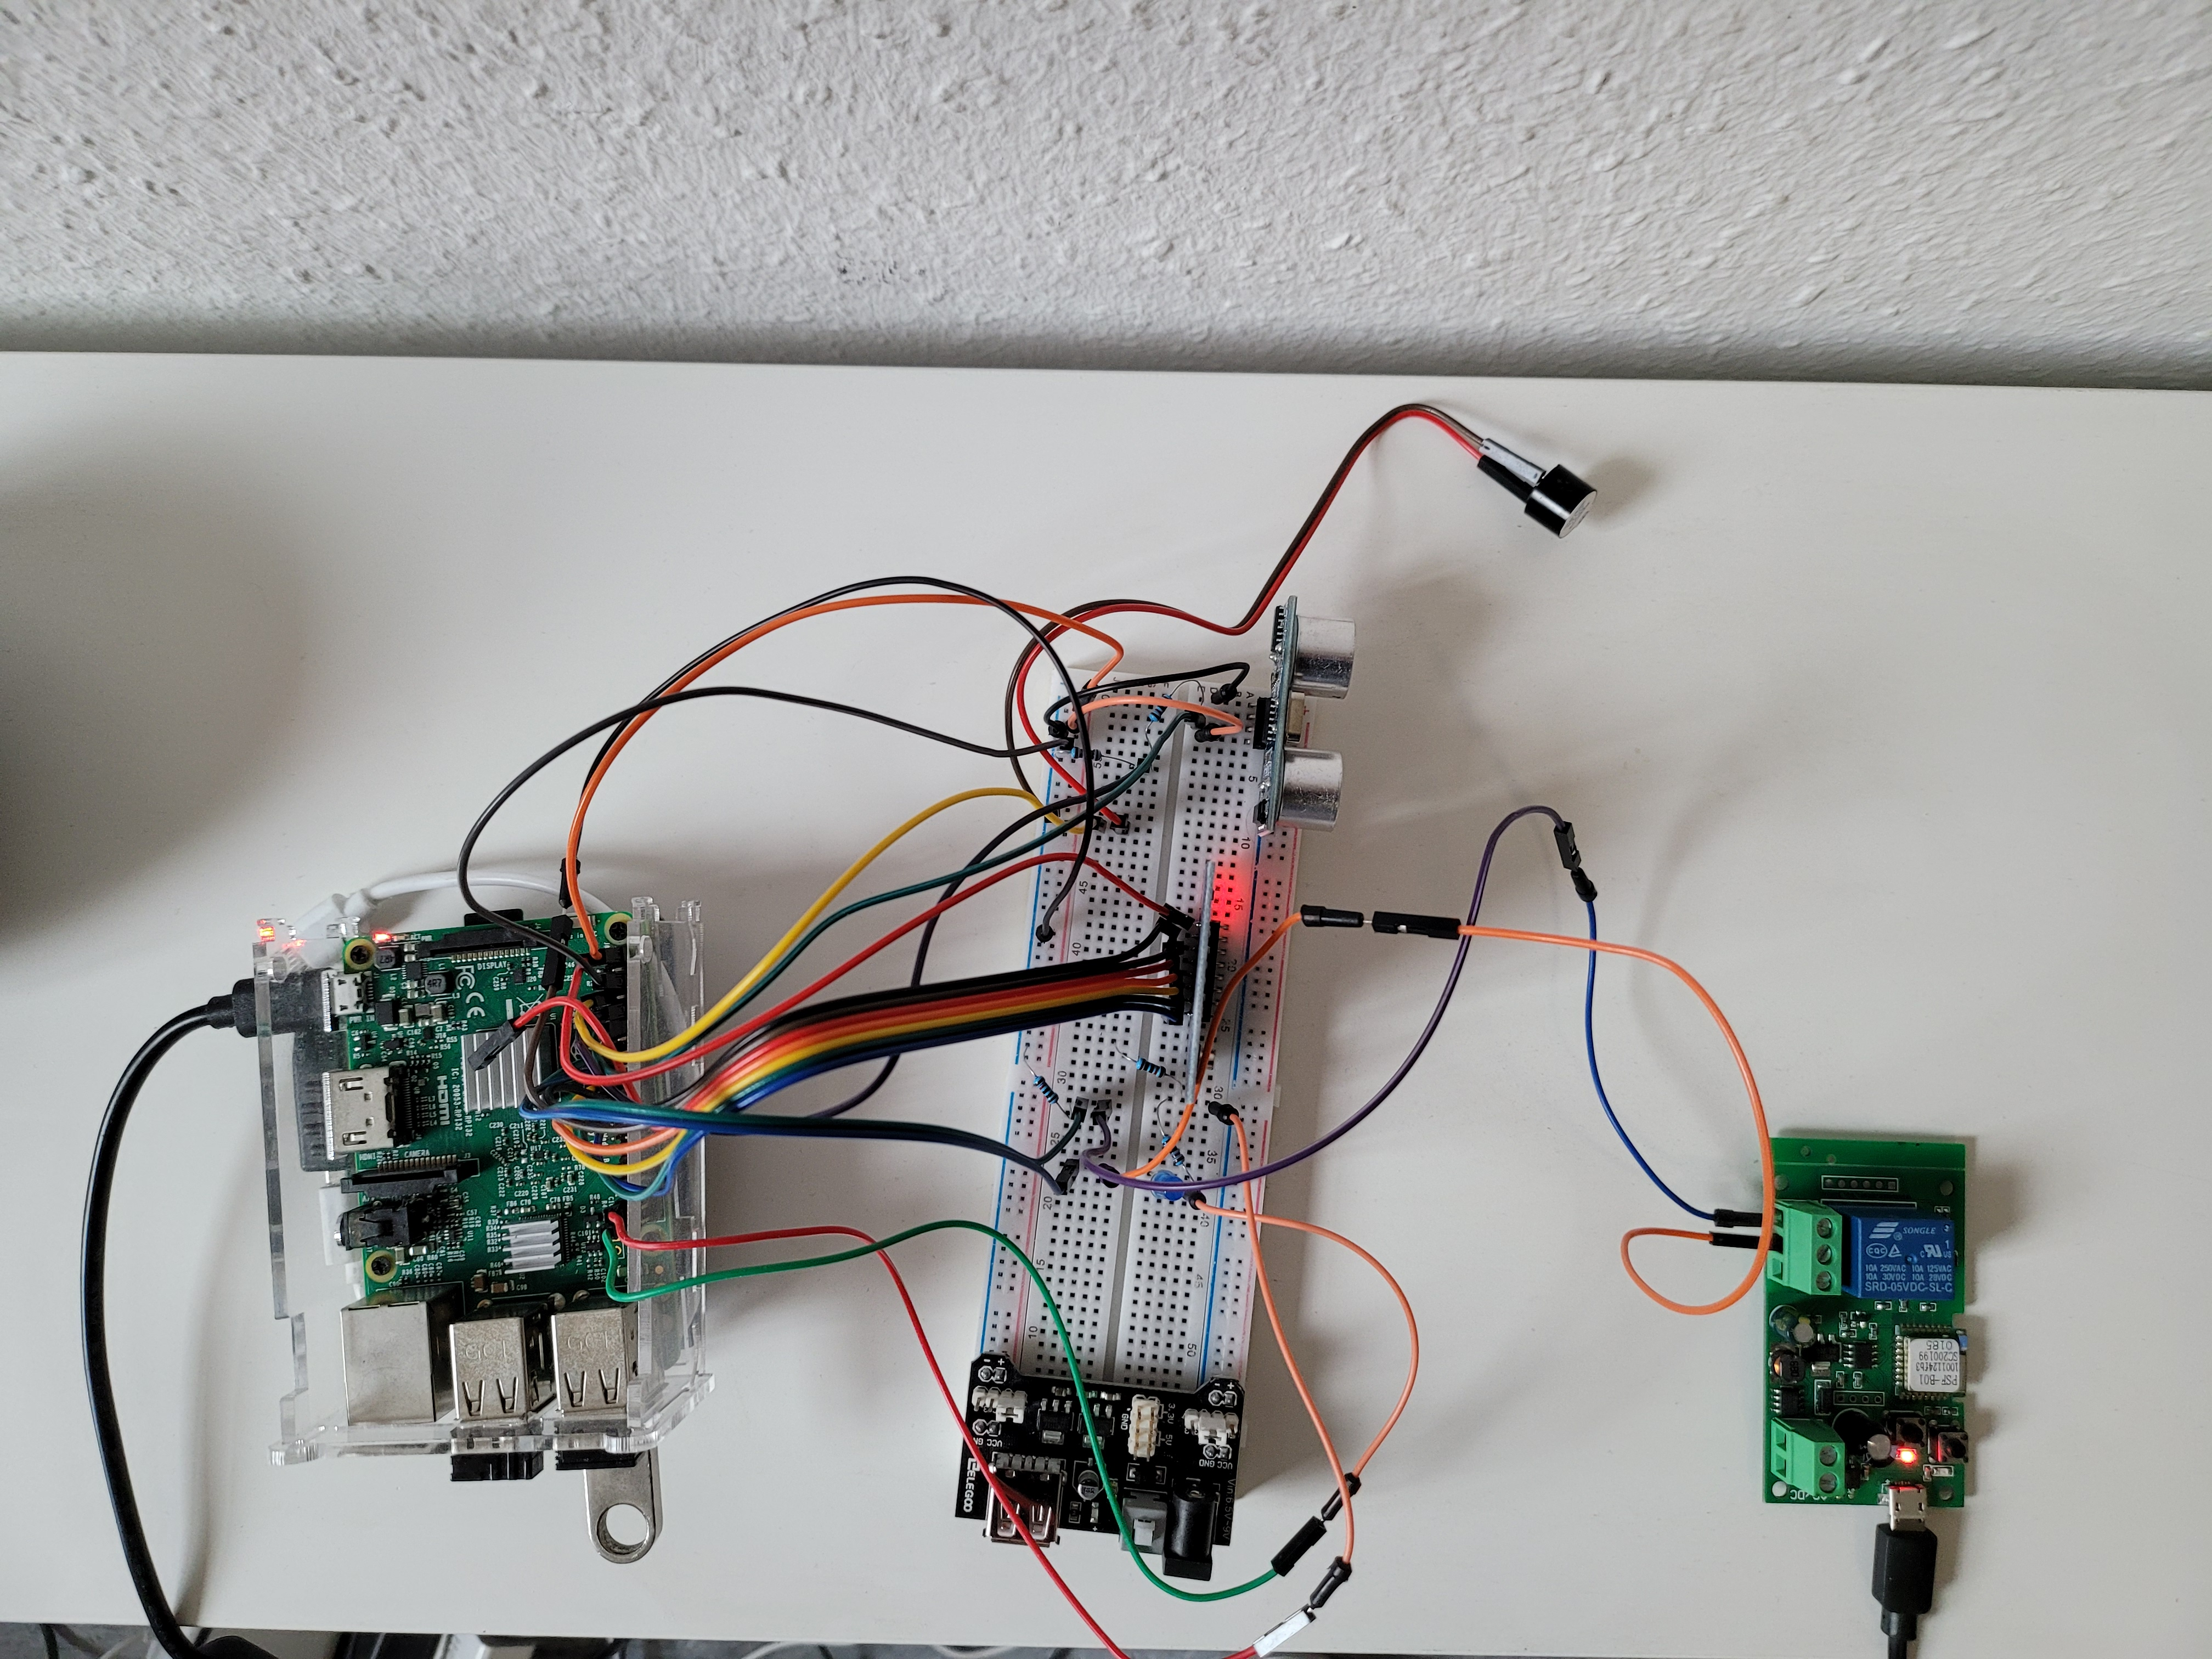
\includegraphics[scale=0.08]{\imagedir/Foto (1).jpg}
	\captionsetup{format=hang}
	\caption[Foto Aufbau 1]{\label{}Raspberry Pi, Breadboard und Alexa-Modul\\Quelle: Eigene Darstellung}
\end{figure}
\begin{figure}
	\centering 
	\label{Aufbau2}
	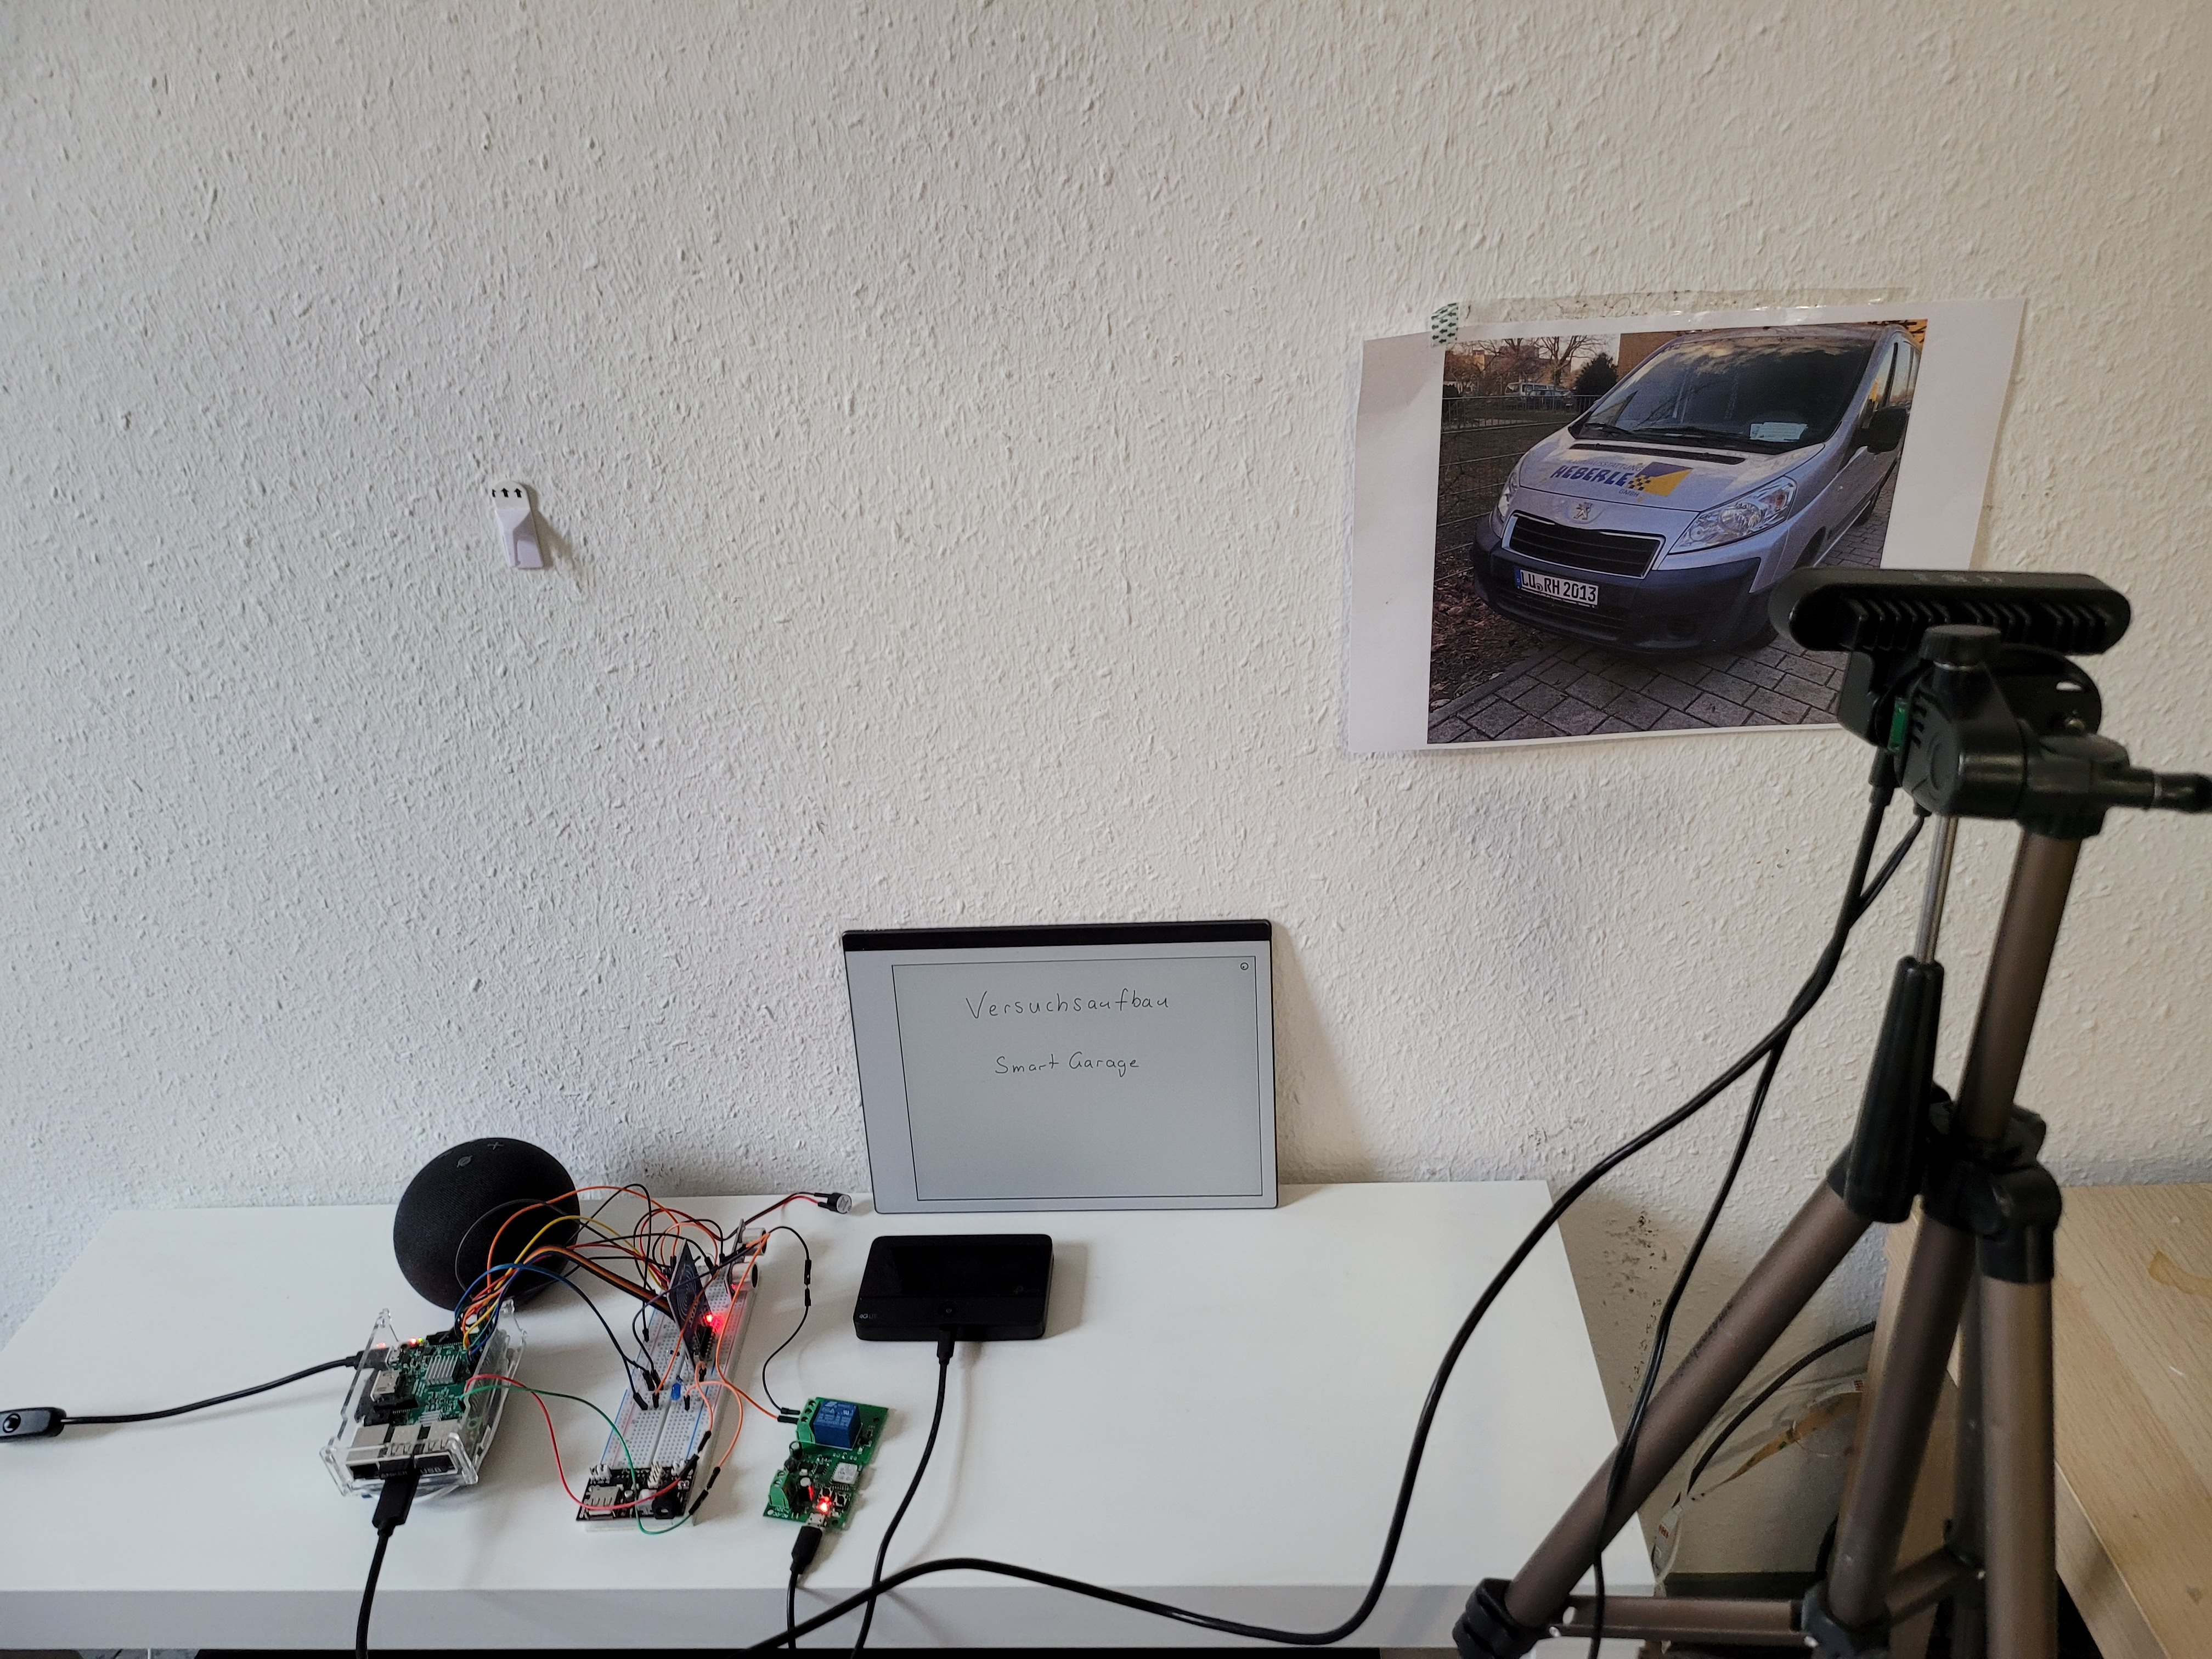
\includegraphics[scale=0.08]{\imagedir/Foto (2).jpg}
	\captionsetup{format=hang}
	\caption[Foto Aufbau 2]{\label{Aufbauanhang}Aufbau mit Kamera \\Quelle: Eigene Darstellung}
\end{figure}
\begin{figure}
	\centering 
	\label{Aufbau3}
	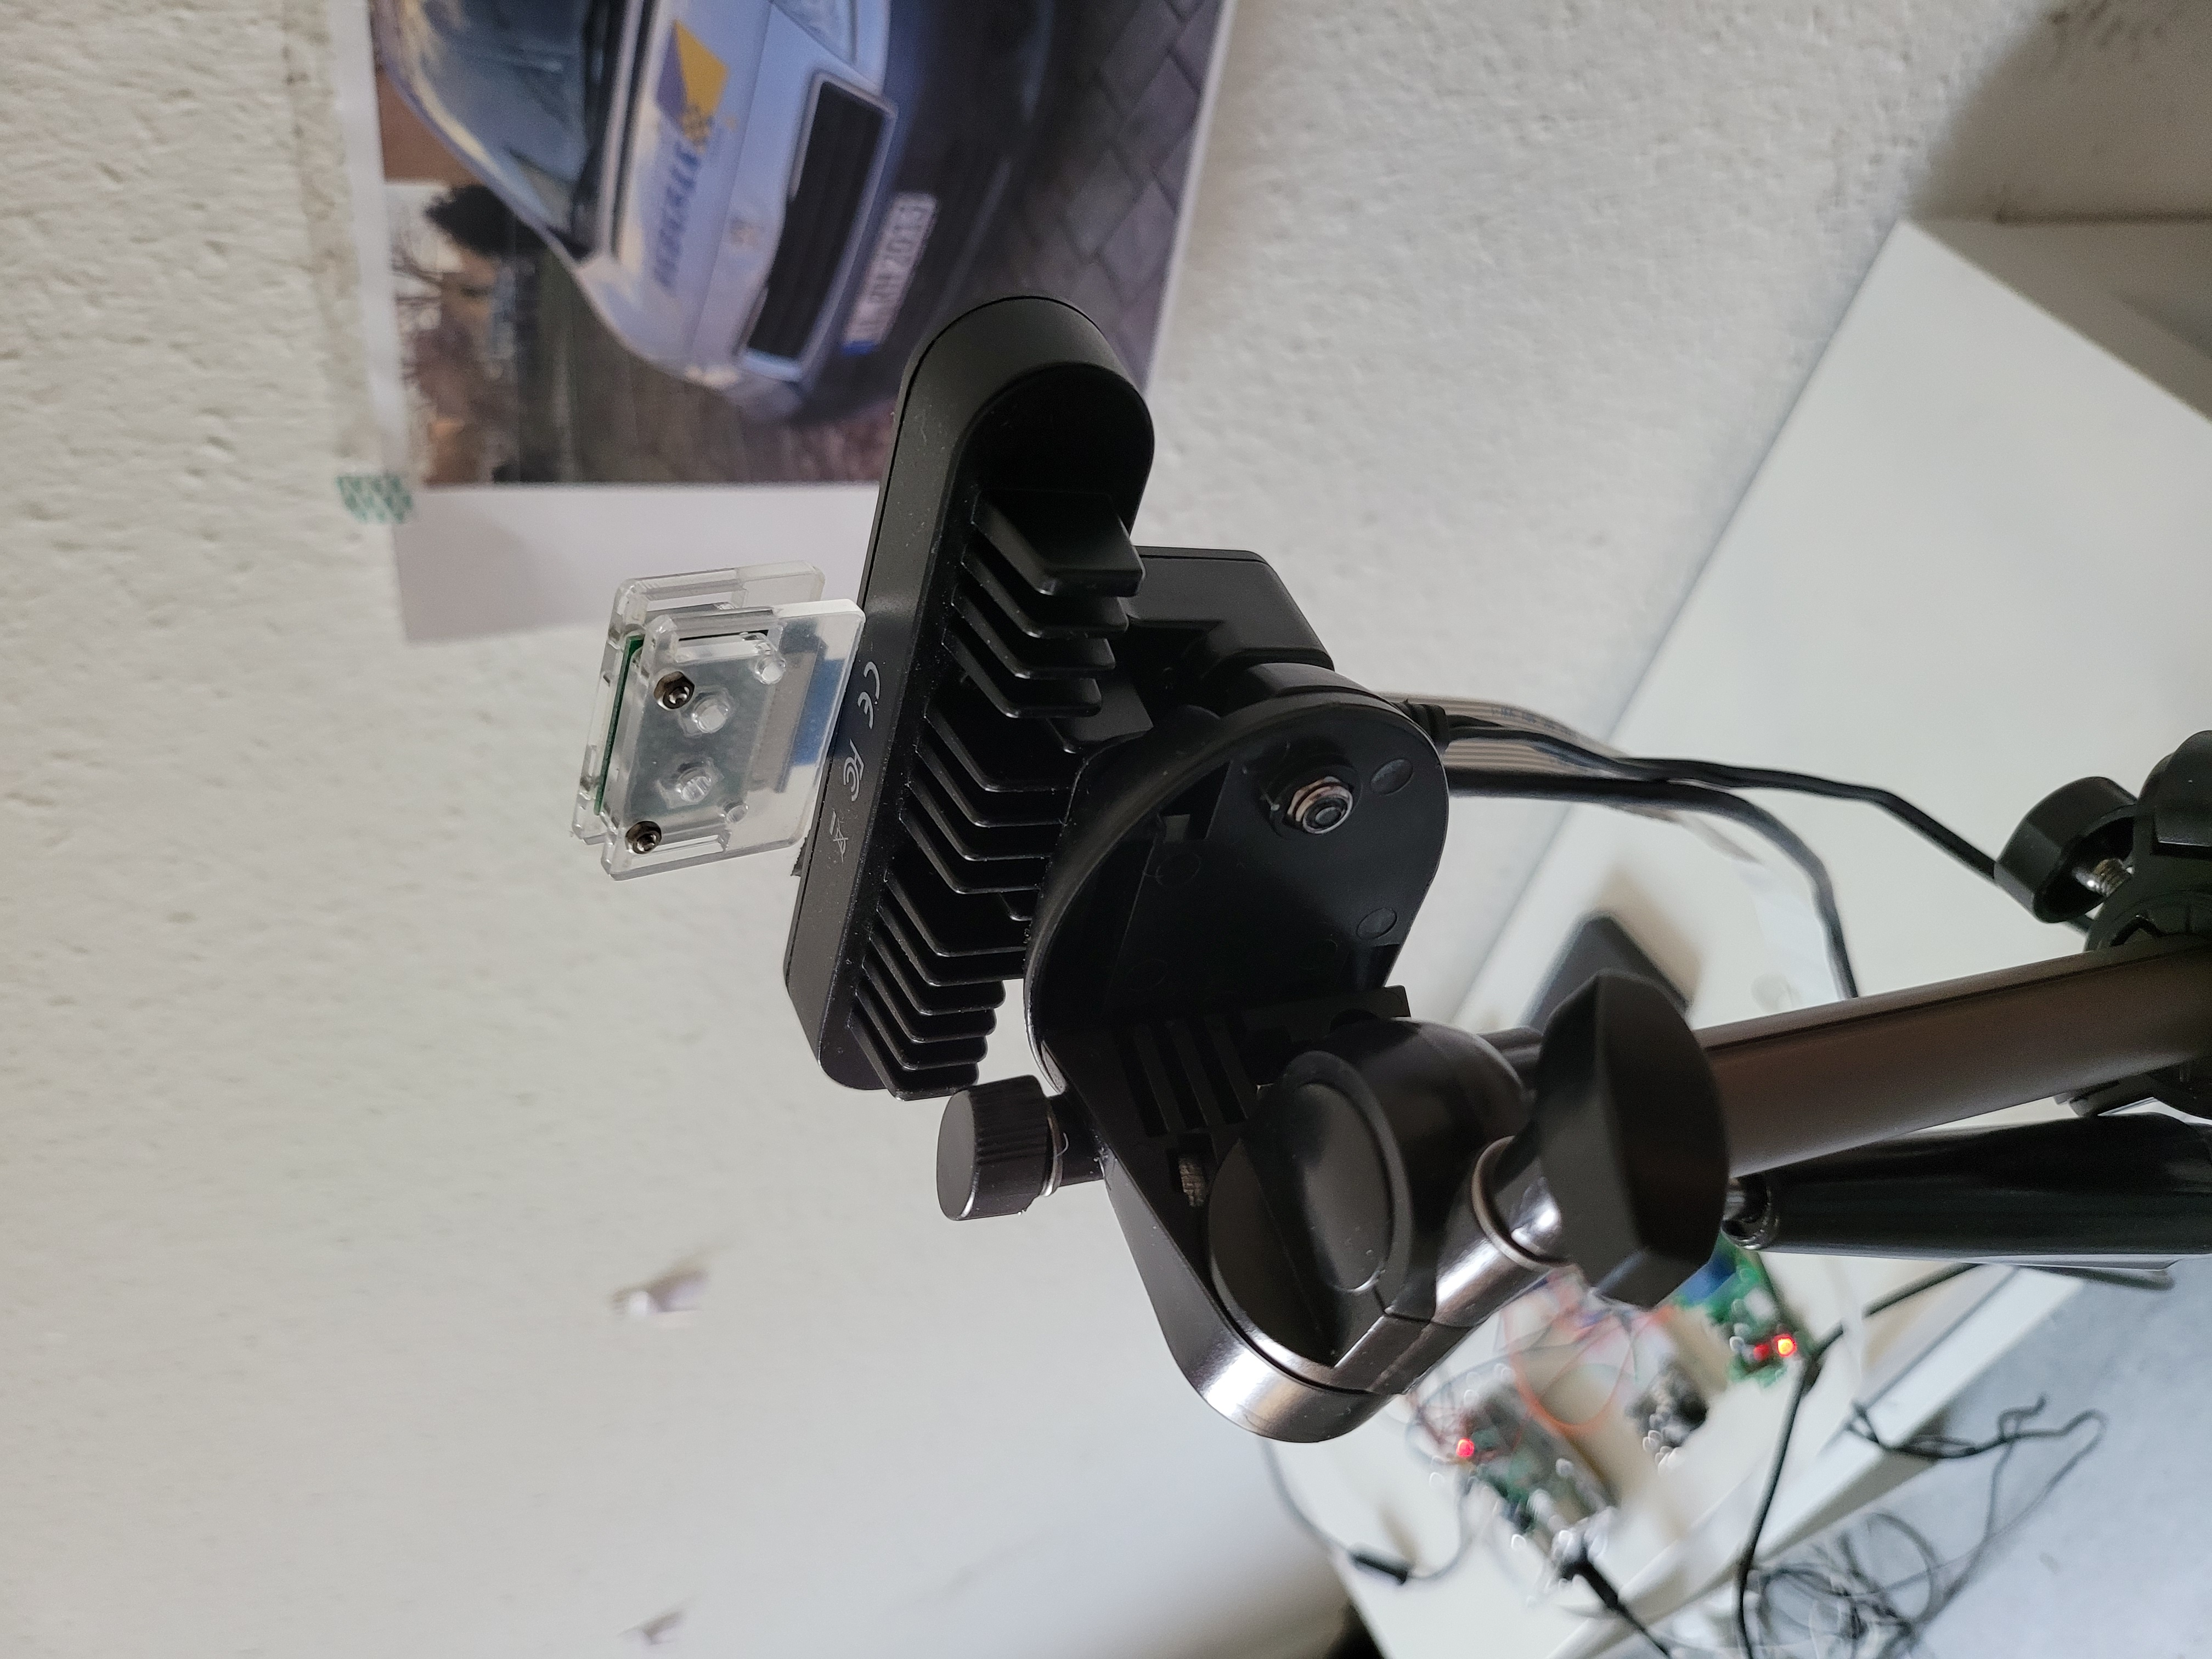
\includegraphics[scale=0.08]{\imagedir/Foto (3).jpg}
	\captionsetup{format=hang}
	\caption[Foto Aufbau 3]{\label{}Notlösung mit Raspi-Kamera nach Defekt \\Quelle: Eigene Darstellung}
\end{figure}
%\begin{figure}
%	\centering 
%	\label{Aufbau4}
%	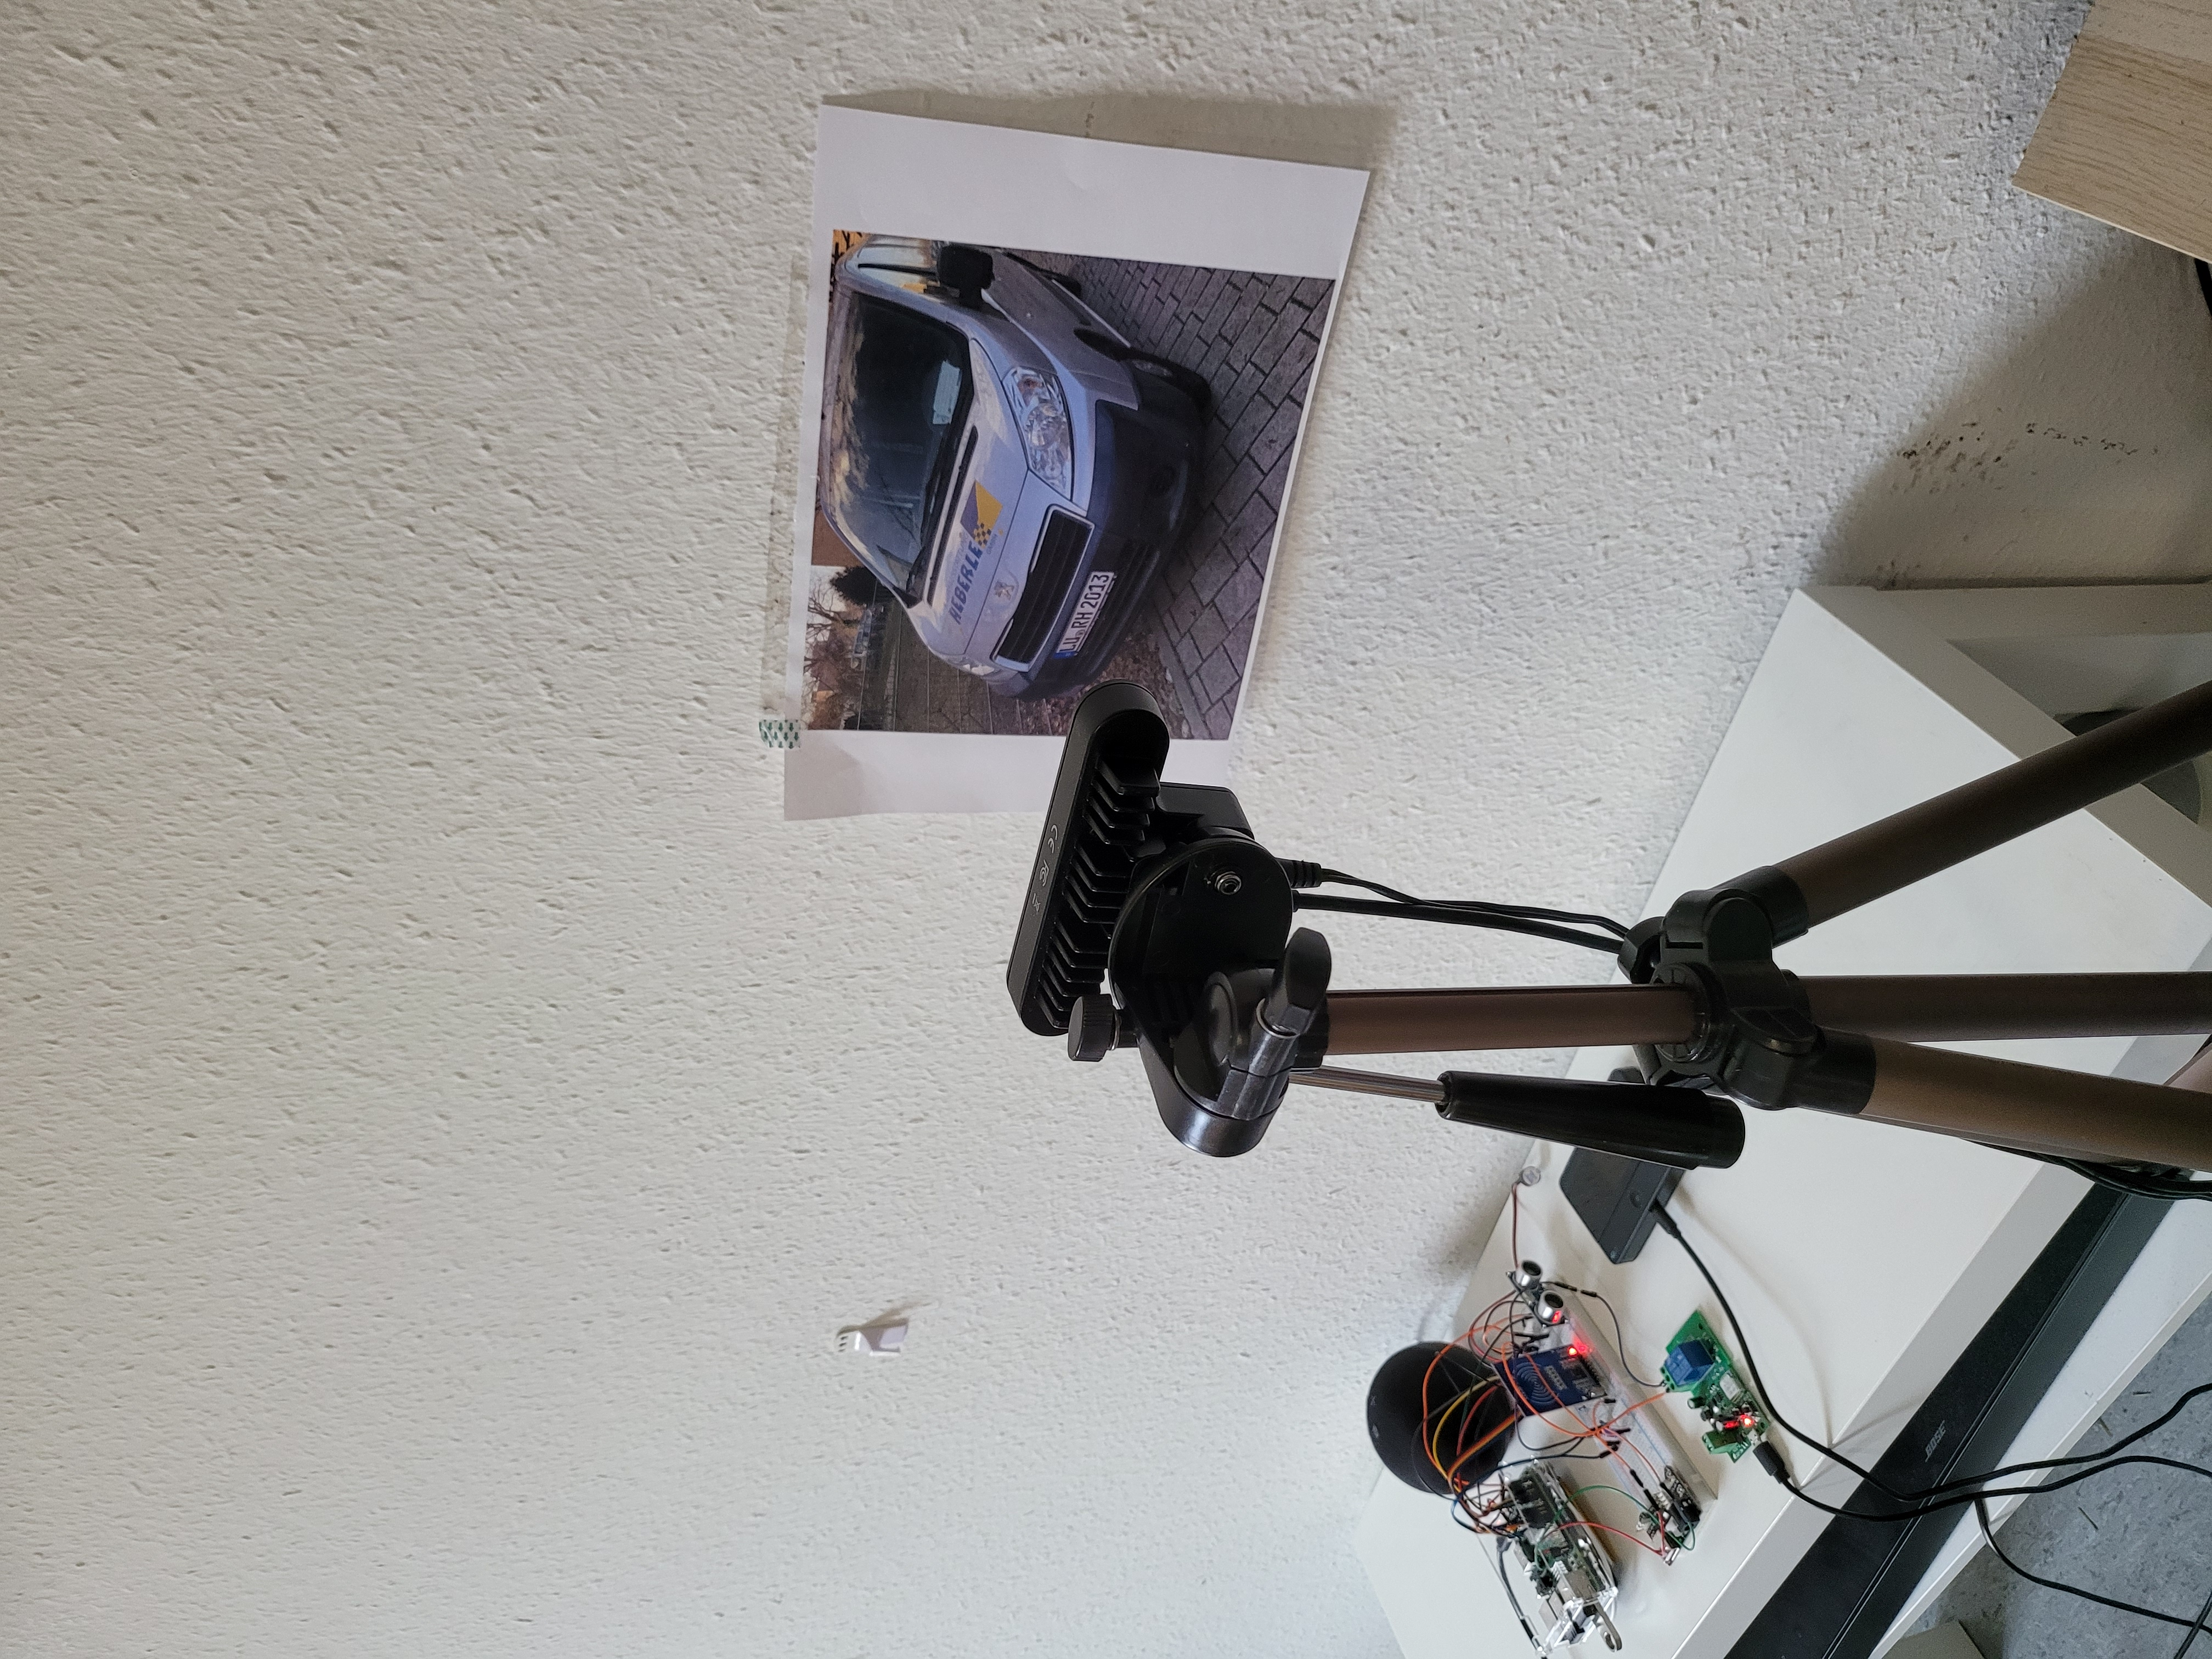
\includegraphics[scale=0.08]{\imagedir/Foto (5).jpg}
%	\captionsetup{format=hang}
%	\caption[Steckplan]{\label{}Steckplan der gesamten Hardware \\Quelle: Eigene Darstellung}
%\end{figure}



\chapter{Fehlermeldungen}
